\documentclass[10pt]{article}
\usepackage[a4paper,margin=1.5cm]{geometry}
\usepackage[T1]{fontenc}\usepackage[utf8]{inputenc}
\usepackage{amsmath,amssymb,tikz,xcolor,adjustbox}
\pagestyle{empty}\setlength\parindent{0pt}
\begin{document}
\section*{Stufe 1 – Hypotenuse oder Kathete erkennen}
\begin{minipage}[t]{\linewidth}
\parbox[t]{5.8cm}{\adjustbox{max width=5.5cm,max height=4.2cm,valign=t}{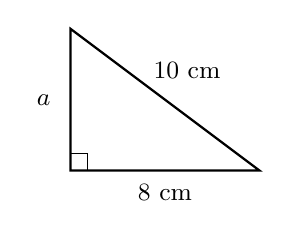
\begin{tikzpicture}[thick]
\draw (0,0)--(2.4,0)--(0,1.8)--cycle;
\draw[thin] (0.22,0)--(0.22,0.22)--(0,0.22);
\node at (1.2,-0.28) {\small 8 cm};
\node at (-0.34,0.9) {\small $a$};
\node at (1.48,1.27) {\small 10 cm};
\end{tikzpicture}}}\hfill\parbox[t]{11.6cm}{\textbf{001}\quad Ist die gesuchte Seite Hypotenuse oder Kathete? Kreise H oder K ein.\\[2pt]{\color{gray}\footnotesize erkennen · lage-standard, gesucht-kathete, abc · basis\\Ergebnis: K}}
\end{minipage}\par\medskip\hrule\medskip
\begin{minipage}[t]{\linewidth}
\parbox[t]{5.8cm}{\adjustbox{max width=5.5cm,max height=4.2cm,valign=t}{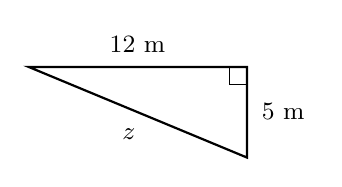
\begin{tikzpicture}[thick]
\draw (2.77,1.15)--(0,1.15)--(2.77,0)--cycle;
\draw[thin] (2.55,1.15)--(2.55,0.93)--(2.77,0.93);
\node at (1.38,1.43) {\small 12 m};
\node at (3.23,0.58) {\small 5 m};
\node at (1.27,0.3) {\small $z$};
\end{tikzpicture}}}\hfill\parbox[t]{11.6cm}{\textbf{002}\quad Ist die gesuchte Seite Hypotenuse oder Kathete? Kreise H oder K ein.\\[2pt]{\color{gray}\footnotesize erkennen · lage-gedreht, gesucht-hyp, andere-buchstaben · basis\\Ergebnis: H}}
\end{minipage}\par\medskip\hrule\medskip
\begin{minipage}[t]{\linewidth}
\parbox[t]{5.8cm}{\adjustbox{max width=5.5cm,max height=4.2cm,valign=t}{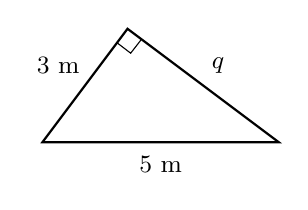
\begin{tikzpicture}[thick]
\draw (1.08,1.44)--(0,0)--(3,0)--cycle;
\draw[thin] (0.95,1.26)--(1.12,1.13)--(1.26,1.31);
\node at (0.2,0.97) {\small 3 m};
\node at (2.23,0.97) {\small $q$};
\node at (1.5,-0.28) {\small 5 m};
\end{tikzpicture}}}\hfill\parbox[t]{11.6cm}{\textbf{003}\quad Ist die gesuchte Seite Hypotenuse oder Kathete? Kreise H oder K ein.\\[2pt]{\color{gray}\footnotesize erkennen · hyp-waagerecht, gesucht-kathete, andere-buchstaben · basis\\Ergebnis: K}}
\end{minipage}\par\medskip\hrule\medskip
\begin{minipage}[t]{\linewidth}
\parbox[t]{5.8cm}{\adjustbox{max width=5.5cm,max height=4.2cm,valign=t}{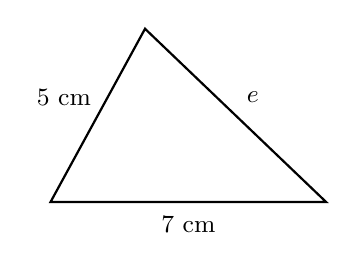
\begin{tikzpicture}[thick]
\draw (0,0)--(3.5,0)--(1.2,2.2)--cycle;
\node at (1.75,-0.28) {\small 7 cm};
\node at (0.17,1.33) {\small 5 cm};
\node at (2.57,1.33) {\small $e$};
\end{tikzpicture}}}\hfill\parbox[t]{11.6cm}{\textbf{004}\quad Ist die gesuchte Seite Hypotenuse oder Kathete? Kreise H oder K ein.\\[2pt]{\color{gray}\footnotesize erkennen · kein-rechter-winkel, andere-buchstaben · basis\\Ergebnis: weder}}
\end{minipage}\par\medskip\hrule\medskip
\begin{minipage}[t]{\linewidth}
\parbox[t]{5.8cm}{\adjustbox{max width=5.5cm,max height=4.2cm,valign=t}{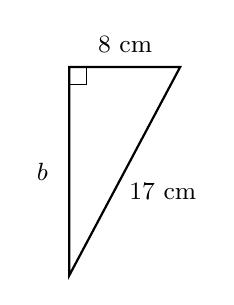
\begin{tikzpicture}[thick]
\draw (0,2.65)--(0,0)--(1.41,2.65)--cycle;
\draw[thin] (0,2.43)--(0.22,2.43)--(0.22,2.65);
\node at (-0.34,1.32) {\small $b$};
\node at (0.71,2.93) {\small 8 cm};
\node at (1.19,1.07) {\small 17 cm};
\end{tikzpicture}}}\hfill\parbox[t]{11.6cm}{\textbf{005}\quad Ist die gesuchte Seite Hypotenuse oder Kathete? Kreise H oder K ein.\\[2pt]{\color{gray}\footnotesize erkennen · lage-gedreht, gesucht-kathete, abc · basis\\Ergebnis: K}}
\end{minipage}\par\medskip\hrule\medskip
\begin{minipage}[t]{\linewidth}
\parbox[t]{5.8cm}{\adjustbox{max width=5.5cm,max height=4.2cm,valign=t}{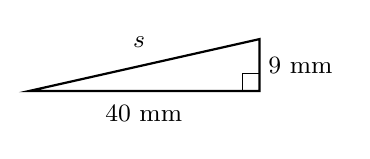
\begin{tikzpicture}[thick]
\draw (2.93,0)--(0,0)--(2.93,0.66)--cycle;
\draw[thin] (2.71,0)--(2.71,0.22)--(2.93,0.22);
\node at (1.46,-0.28) {\small 40 mm};
\node at (3.45,0.33) {\small 9 mm};
\node at (1.4,0.62) {\small $s$};
\end{tikzpicture}}}\hfill\parbox[t]{11.6cm}{\textbf{006}\quad Ist die gesuchte Seite Hypotenuse oder Kathete? Kreise H oder K ein.\\[2pt]{\color{gray}\footnotesize erkennen · lage-gedreht, gesucht-hyp, andere-buchstaben · basis\\Ergebnis: H}}
\end{minipage}\par\medskip\hrule\medskip
\begin{minipage}[t]{\linewidth}
\parbox[t]{5.8cm}{\adjustbox{max width=5.5cm,max height=4.2cm,valign=t}{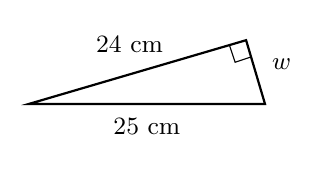
\begin{tikzpicture}[thick]
\draw (2.76,0.81)--(0,0)--(3,0)--cycle;
\draw[thin] (2.55,0.74)--(2.62,0.53)--(2.83,0.6);
\node at (1.28,0.75) {\small 24 cm};
\node at (3.21,0.5) {\small $w$};
\node at (1.5,-0.28) {\small 25 cm};
\end{tikzpicture}}}\hfill\parbox[t]{11.6cm}{\textbf{007}\quad Ist die gesuchte Seite Hypotenuse oder Kathete? Kreise H oder K ein.\\[2pt]{\color{gray}\footnotesize erkennen · hyp-waagerecht, gesucht-kathete, andere-buchstaben · basis\\Ergebnis: K}}
\end{minipage}\par\medskip\hrule\medskip
\begin{minipage}[t]{\linewidth}
\parbox[t]{5.8cm}{\adjustbox{max width=5.5cm,max height=4.2cm,valign=t}{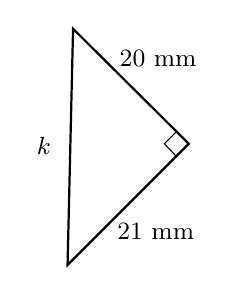
\begin{tikzpicture}[thick]
\draw (1.54,1.54)--(0.07,3)--(0,0)--cycle;
\draw[thin] (1.38,1.69)--(1.23,1.54)--(1.38,1.38);
\node at (1.15,2.62) {\small 20 mm};
\node at (1.12,0.42) {\small 21 mm};
\node at (-0.3,1.51) {\small $k$};
\end{tikzpicture}}}\hfill\parbox[t]{11.6cm}{\textbf{008}\quad Ist die gesuchte Seite Hypotenuse oder Kathete? Kreise H oder K ein.\\[2pt]{\color{gray}\footnotesize erkennen · lage-gedreht, gesucht-hyp, andere-buchstaben · basis\\Ergebnis: H}}
\end{minipage}\par\medskip\hrule\medskip
\begin{minipage}[t]{\linewidth}
\parbox[t]{5.8cm}{\adjustbox{max width=5.5cm,max height=4.2cm,valign=t}{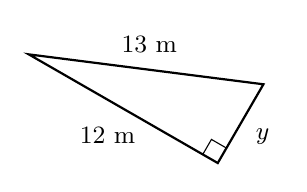
\begin{tikzpicture}[thick]
\draw (2.4,0)--(2.98,1)--(0,1.38)--cycle;
\draw[thin] (2.51,0.19)--(2.32,0.3)--(2.21,0.11);
\node at (2.97,0.33) {\small $y$};
\node at (1,0.35) {\small 12 m};
\node at (1.53,1.5) {\small 13 m};
\end{tikzpicture}}}\hfill\parbox[t]{11.6cm}{\textbf{009}\quad Ist die gesuchte Seite Hypotenuse oder Kathete? Kreise H oder K ein.\\[2pt]{\color{gray}\footnotesize erkennen · lage-gedreht, gesucht-kathete, andere-buchstaben · basis\\Ergebnis: K}}
\end{minipage}\par\medskip\hrule\medskip
\begin{minipage}[t]{\linewidth}
\parbox[t]{5.8cm}{\adjustbox{max width=5.5cm,max height=4.2cm,valign=t}{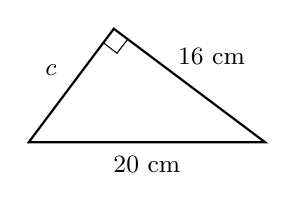
\begin{tikzpicture}[thick]
\draw (1.08,1.44)--(0,0)--(3,0)--cycle;
\draw[thin] (0.95,1.26)--(1.12,1.13)--(1.26,1.31);
\node at (0.28,0.92) {\small $c$};
\node at (2.32,1.09) {\small 16 cm};
\node at (1.5,-0.28) {\small 20 cm};
\end{tikzpicture}}}\hfill\parbox[t]{11.6cm}{\textbf{010}\quad Ist die gesuchte Seite Hypotenuse oder Kathete? Kreise H oder K ein.\\[2pt]{\color{gray}\footnotesize erkennen · hyp-waagerecht, gesucht-kathete, abc · basis\\Ergebnis: K}}
\end{minipage}\par\medskip\hrule\medskip
\clearpage
\section*{Stufe 2 – Satz umgestellt notieren}
\begin{minipage}[t]{\linewidth}
\parbox[t]{5.8cm}{\parbox[t]{5.5cm}{\color{gray}\small (ohne Skizze)}}\hfill\parbox[t]{11.6cm}{\textbf{011}\quad Notiere den Satz des Pythagoras nach einer Kathete umgestellt. Verwende eine Skizze. Schlage im Tafelwerk nach und trage die Seite ein: S.~\rule{1.2cm}{0.4pt}\\[2pt]{\color{gray}\footnotesize notieren · – · basis\\Ergebnis: $a^2 = c^2 - b^2$, $b^2 = c^2 - a^2$}}
\end{minipage}\par\medskip\hrule\medskip
\begin{minipage}[t]{\linewidth}
\parbox[t]{5.8cm}{\parbox[t]{5.5cm}{\color{gray}\small (ohne Skizze)}}\hfill\parbox[t]{11.6cm}{\textbf{012}\quad Notiere den Satz des Pythagoras nach jeder der beiden Katheten umgestellt. Verwende eine Skizze mit den Seiten $r$, $s$ und $t$; $t$ ist die Hypotenuse.\\[2pt]{\color{gray}\footnotesize notieren · – · basis\\Ergebnis: $r^2 = t^2 - s^2$, $s^2 = t^2 - r^2$}}
\end{minipage}\par\medskip\hrule\medskip
\clearpage
\section*{Stufe 3 – Gleichung aufstellen}
\begin{minipage}[t]{\linewidth}
\parbox[t]{5.8cm}{\adjustbox{max width=5.5cm,max height=4.2cm,valign=t}{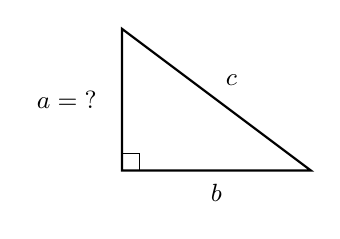
\begin{tikzpicture}[thick]
\draw (0,0)--(2.4,0)--(0,1.8)--cycle;
\draw[thin] (0.22,0)--(0.22,0.22)--(0,0.22);
\node at (1.2,-0.28) {\small $b$};
\node at (-0.7,0.9) {\small $a = {?}$};
\node at (1.39,1.15) {\small $c$};
\end{tikzpicture}}}\hfill\parbox[t]{11.6cm}{\textbf{013}\quad Stelle die Gleichung für die gesuchte Seite auf. Rechne nicht.\\[2pt]{\color{gray}\footnotesize aufstellen · lage-standard, gesucht-kathete, abc · basis\\Ergebnis: $a^2 = c^2 - b^2$}}
\end{minipage}\par\medskip\hrule\medskip
\begin{minipage}[t]{\linewidth}
\parbox[t]{5.8cm}{\adjustbox{max width=5.5cm,max height=4.2cm,valign=t}{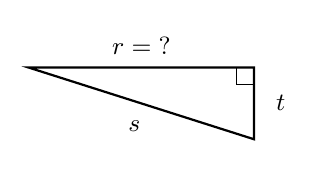
\begin{tikzpicture}[thick]
\draw (2.86,0.91)--(0,0.91)--(2.86,0)--cycle;
\draw[thin] (2.64,0.91)--(2.64,0.69)--(2.86,0.69);
\node at (1.43,1.19) {\small $r = {?}$};
\node at (3.2,0.46) {\small $t$};
\node at (1.34,0.17) {\small $s$};
\end{tikzpicture}}}\hfill\parbox[t]{11.6cm}{\textbf{014}\quad Stelle die Gleichung für die gesuchte Seite auf. Rechne nicht.\\[2pt]{\color{gray}\footnotesize aufstellen · lage-gedreht, gesucht-kathete, andere-buchstaben · basis\\Ergebnis: $r^2 = s^2 - t^2$}}
\end{minipage}\par\medskip\hrule\medskip
\begin{minipage}[t]{\linewidth}
\parbox[t]{5.8cm}{\adjustbox{max width=5.5cm,max height=4.2cm,valign=t}{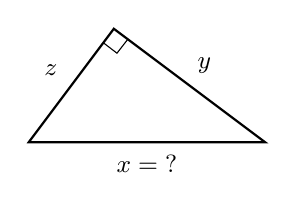
\begin{tikzpicture}[thick]
\draw (1.08,1.44)--(0,0)--(3,0)--cycle;
\draw[thin] (0.95,1.26)--(1.12,1.13)--(1.26,1.31);
\node at (0.28,0.92) {\small $z$};
\node at (2.23,0.97) {\small $y$};
\node at (1.5,-0.28) {\small $x = {?}$};
\end{tikzpicture}}}\hfill\parbox[t]{11.6cm}{\textbf{015}\quad Stelle die Gleichung für die gesuchte Seite auf. Rechne nicht.\\[2pt]{\color{gray}\footnotesize aufstellen · hyp-waagerecht, gesucht-hyp, andere-buchstaben · basis\\Ergebnis: $x^2 = z^2 + y^2$}}
\end{minipage}\par\medskip\hrule\medskip
\begin{minipage}[t]{\linewidth}
\parbox[t]{5.8cm}{\adjustbox{max width=5.5cm,max height=4.2cm,valign=t}{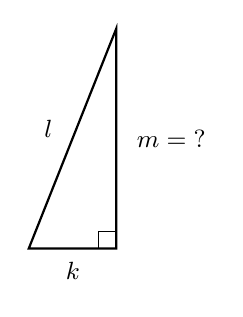
\begin{tikzpicture}[thick]
\draw (1.11,0)--(0,0)--(1.11,2.79)--cycle;
\draw[thin] (0.89,0)--(0.89,0.22)--(1.11,0.22);
\node at (0.56,-0.28) {\small $k$};
\node at (1.81,1.39) {\small $m = {?}$};
\node at (0.25,1.52) {\small $l$};
\end{tikzpicture}}}\hfill\parbox[t]{11.6cm}{\textbf{016}\quad Stelle die Gleichung für die gesuchte Seite auf. Rechne nicht.\\[2pt]{\color{gray}\footnotesize aufstellen · lage-gedreht, gesucht-kathete, andere-buchstaben · basis\\Ergebnis: $m^2 = l^2 - k^2$}}
\end{minipage}\par\medskip\hrule\medskip
\begin{minipage}[t]{\linewidth}
\parbox[t]{5.8cm}{\adjustbox{max width=5.5cm,max height=4.2cm,valign=t}{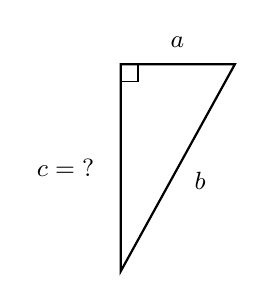
\begin{tikzpicture}[thick]
\draw (0,2.63)--(0,0)--(1.45,2.63)--cycle;
\draw[thin] (0,2.41)--(0.22,2.41)--(0.22,2.63);
\node at (-0.7,1.31) {\small $c = {?}$};
\node at (0.72,2.91) {\small $a$};
\node at (1.01,1.15) {\small $b$};
\end{tikzpicture}}}\hfill\parbox[t]{11.6cm}{\textbf{017}\quad Stelle die Gleichung für die gesuchte Seite auf. Rechne nicht.\\[2pt]{\color{gray}\footnotesize aufstellen · lage-gedreht, gesucht-kathete, abc · basis\\Ergebnis: $c^2 = b^2 - a^2$}}
\end{minipage}\par\medskip\hrule\medskip
\begin{minipage}[t]{\linewidth}
\parbox[t]{5.8cm}{\adjustbox{max width=5.5cm,max height=4.2cm,valign=t}{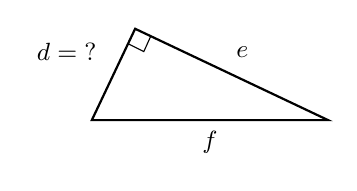
\begin{tikzpicture}[thick]
\draw (0.55,1.16)--(0,0)--(3,0)--cycle;
\draw[thin] (0.46,0.97)--(0.66,0.87)--(0.75,1.07);
\node at (-0.32,0.87) {\small $d = {?}$};
\node at (1.91,0.86) {\small $e$};
\node at (1.5,-0.28) {\small $f$};
\end{tikzpicture}}}\hfill\parbox[t]{11.6cm}{\textbf{018}\quad Stelle die Gleichung für die gesuchte Seite auf. Rechne nicht.\\[2pt]{\color{gray}\footnotesize aufstellen · hyp-waagerecht, gesucht-kathete, andere-buchstaben · basis\\Ergebnis: $d^2 = f^2 - e^2$}}
\end{minipage}\par\medskip\hrule\medskip
\begin{minipage}[t]{\linewidth}
\parbox[t]{5.8cm}{\adjustbox{max width=5.5cm,max height=4.2cm,valign=t}{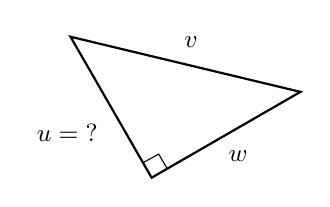
\begin{tikzpicture}[thick]
\draw (1.03,0)--(2.92,1.09)--(0,1.79)--cycle;
\draw[thin] (1.23,0.11)--(1.12,0.3)--(0.92,0.19);
\node at (2.13,0.27) {\small $w$};
\node at (-0.04,0.57) {\small $u = {?}$};
\node at (1.53,1.72) {\small $v$};
\end{tikzpicture}}}\hfill\parbox[t]{11.6cm}{\textbf{019}\quad Stelle die Gleichung für die gesuchte Seite auf. Rechne nicht.\\[2pt]{\color{gray}\footnotesize aufstellen · lage-gedreht, gesucht-kathete, andere-buchstaben · basis\\Ergebnis: $u^2 = v^2 - w^2$}}
\end{minipage}\par\medskip\hrule\medskip
\begin{minipage}[t]{\linewidth}
\parbox[t]{5.8cm}{\adjustbox{max width=5.5cm,max height=4.2cm,valign=t}{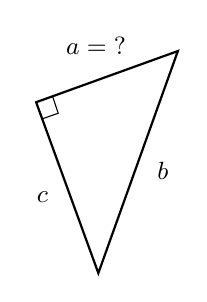
\begin{tikzpicture}[thick]
\draw (0,2.17)--(1.8,2.82)--(0.79,0)--cycle;
\draw[thin] (0.21,2.24)--(0.28,2.03)--(0.08,1.96);
\node at (0.76,2.89) {\small $a = {?}$};
\node at (0.08,0.97) {\small $c$};
\node at (1.61,1.3) {\small $b$};
\end{tikzpicture}}}\hfill\parbox[t]{11.6cm}{\textbf{020}\quad Stelle die Gleichung für die gesuchte Seite auf. Rechne nicht.\\[2pt]{\color{gray}\footnotesize aufstellen · lage-gedreht, gesucht-kathete, abc · basis\\Ergebnis: $a^2 = b^2 - c^2$}}
\end{minipage}\par\medskip\hrule\medskip
\begin{minipage}[t]{\linewidth}
\parbox[t]{5.8cm}{\adjustbox{max width=5.5cm,max height=4.2cm,valign=t}{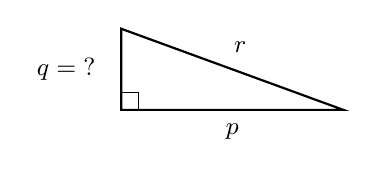
\begin{tikzpicture}[thick]
\draw (0,0)--(2.82,0)--(0,1.03)--cycle;
\draw[thin] (0.22,0)--(0.22,0.22)--(0,0.22);
\node at (1.41,-0.28) {\small $p$};
\node at (-0.7,0.51) {\small $q = {?}$};
\node at (1.51,0.8) {\small $r$};
\end{tikzpicture}}}\hfill\parbox[t]{11.6cm}{\textbf{021}\quad Stelle die Gleichung für die gesuchte Seite auf. Rechne nicht.\\[2pt]{\color{gray}\footnotesize aufstellen · lage-standard, gesucht-kathete, andere-buchstaben · basis\\Ergebnis: $q^2 = r^2 - p^2$}}
\end{minipage}\par\medskip\hrule\medskip
\clearpage
\section*{Stufe 4 – Berechnen (Tripel, Päckchen)}
\begin{minipage}[t]{\linewidth}
\parbox[t]{5.8cm}{\adjustbox{max width=5.5cm,max height=4.2cm,valign=t}{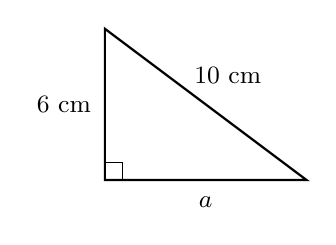
\begin{tikzpicture}[thick]
\draw (0,0)--(2.56,0)--(0,1.92)--cycle;
\draw[thin] (0.22,0)--(0.22,0.22)--(0,0.22);
\node at (1.28,-0.28) {\small $a$};
\node at (-0.52,0.96) {\small 6 cm};
\node at (1.56,1.33) {\small 10 cm};
\end{tikzpicture}}}\hfill\parbox[t]{11.6cm}{\textbf{022}\quad Berechne die fehlende Seite.\\{\color{gray}\footnotesize a) grau: $a^2 = 10^2 - 6^2$ \quad $a^2 = 64 \quad | \sqrt{\ }$ \quad $a = 8$ cm}\\[2pt]{\color{gray}\footnotesize rechnen · tripel, lage-standard, gesucht-kathete, abc · kern\\Ergebnis: $a = 8$ cm}}
\end{minipage}\par\medskip\hrule\medskip
\begin{minipage}[t]{\linewidth}
\parbox[t]{5.8cm}{\adjustbox{max width=5.5cm,max height=4.2cm,valign=t}{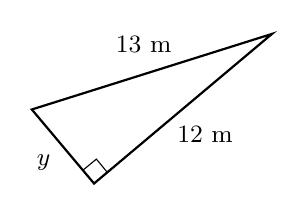
\begin{tikzpicture}[thick]
\draw (0.79,0)--(3.05,1.9)--(0,0.94)--cycle;
\draw[thin] (0.96,0.14)--(0.82,0.31)--(0.65,0.17);
\node at (2.2,0.62) {\small 12 m};
\node at (0.15,0.26) {\small $y$};
\node at (1.42,1.76) {\small 13 m};
\end{tikzpicture}}}\hfill\parbox[t]{11.6cm}{\textbf{023}\quad Berechne die fehlende Seite.\\[2pt]{\color{gray}\footnotesize rechnen · tripel, lage-gedreht, gesucht-kathete, andere-buchstaben · kern\\Ergebnis: $y = 5$ m}}
\end{minipage}\par\medskip\hrule\medskip
\begin{minipage}[t]{\linewidth}
\parbox[t]{5.8cm}{\adjustbox{max width=5.5cm,max height=4.2cm,valign=t}{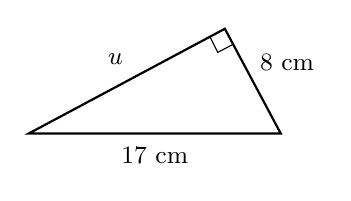
\begin{tikzpicture}[thick]
\draw (2.49,1.33)--(0,0)--(3.2,0)--cycle;
\draw[thin] (2.3,1.23)--(2.4,1.03)--(2.59,1.13);
\node at (1.1,0.94) {\small $u$};
\node at (3.28,0.9) {\small 8 cm};
\node at (1.6,-0.28) {\small 17 cm};
\end{tikzpicture}}}\hfill\parbox[t]{11.6cm}{\textbf{024}\quad Berechne die fehlende Seite.\\[2pt]{\color{gray}\footnotesize rechnen · tripel, hyp-waagerecht, gesucht-kathete, andere-buchstaben · kern\\Ergebnis: $u = 15$ cm}}
\end{minipage}\par\medskip\hrule\medskip
\begin{minipage}[t]{\linewidth}
\parbox[t]{5.8cm}{\adjustbox{max width=5.5cm,max height=4.2cm,valign=t}{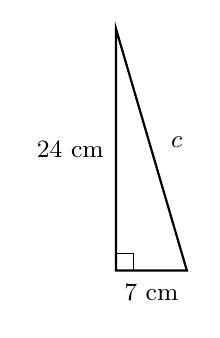
\begin{tikzpicture}[thick]
\draw (0,0)--(0.9,0)--(0,3.07)--cycle;
\draw[thin] (0.22,0)--(0.22,0.22)--(0,0.22);
\node at (0.45,-0.28) {\small 7 cm};
\node at (-0.58,1.54) {\small 24 cm};
\node at (0.77,1.63) {\small $c$};
\end{tikzpicture}}}\hfill\parbox[t]{11.6cm}{\textbf{025}\quad Berechne die fehlende Seite.\\[2pt]{\color{gray}\footnotesize rechnen · tripel, lage-standard, gesucht-hyp, abc · kern\\Ergebnis: $c = 25$ cm}}
\end{minipage}\par\medskip\hrule\medskip
\begin{minipage}[t]{\linewidth}
\parbox[t]{5.8cm}{\adjustbox{max width=5.5cm,max height=4.2cm,valign=t}{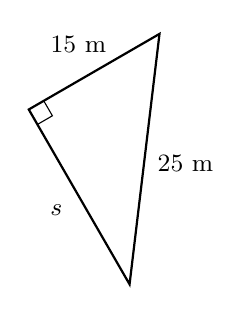
\begin{tikzpicture}[thick]
\draw (0,2.22)--(1.66,3.18)--(1.28,0)--cycle;
\draw[thin] (0.19,2.33)--(0.3,2.14)--(0.11,2.03);
\node at (0.63,3.04) {\small 15 m};
\node at (0.35,0.94) {\small $s$};
\node at (1.99,1.53) {\small 25 m};
\end{tikzpicture}}}\hfill\parbox[t]{11.6cm}{\textbf{026}\quad Berechne die fehlende Seite.\\{\color{gray}\footnotesize a) grau: $s^2 = 25^2 - 15^2$ \quad $s^2 = 400 \quad | \sqrt{\ }$ \quad $s = 20$ m}\\[2pt]{\color{gray}\footnotesize rechnen · tripel, lage-gedreht, gesucht-kathete, andere-buchstaben · kern\\Ergebnis: $s = 20$ m}}
\end{minipage}\par\medskip\hrule\medskip
\begin{minipage}[t]{\linewidth}
\parbox[t]{5.8cm}{\adjustbox{max width=5.5cm,max height=4.2cm,valign=t}{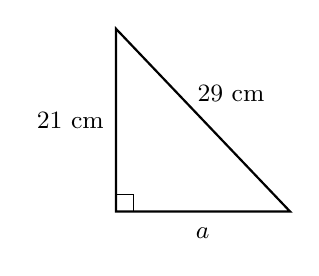
\begin{tikzpicture}[thick]
\draw (0,0)--(2.21,0)--(0,2.32)--cycle;
\draw[thin] (0.22,0)--(0.22,0.22)--(0,0.22);
\node at (1.1,-0.28) {\small $a$};
\node at (-0.58,1.16) {\small 21 cm};
\node at (1.46,1.5) {\small 29 cm};
\end{tikzpicture}}}\hfill\parbox[t]{11.6cm}{\textbf{027}\quad Berechne die fehlende Seite.\\[2pt]{\color{gray}\footnotesize rechnen · tripel, lage-standard, gesucht-kathete, abc · kern\\Ergebnis: $a = 20$ cm}}
\end{minipage}\par\medskip\hrule\medskip
\begin{minipage}[t]{\linewidth}
\parbox[t]{5.8cm}{\adjustbox{max width=5.5cm,max height=4.2cm,valign=t}{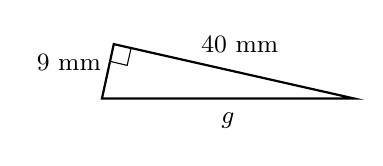
\begin{tikzpicture}[thick]
\draw (0.15,0.69)--(0,0)--(3.2,0)--cycle;
\draw[thin] (0.11,0.47)--(0.32,0.42)--(0.37,0.64);
\node at (-0.42,0.46) {\small 9 mm};
\node at (1.75,0.68) {\small 40 mm};
\node at (1.6,-0.28) {\small $g$};
\end{tikzpicture}}}\hfill\parbox[t]{11.6cm}{\textbf{028}\quad Berechne die fehlende Seite.\\[2pt]{\color{gray}\footnotesize rechnen · tripel, hyp-waagerecht, gesucht-hyp, andere-buchstaben · kern\\Ergebnis: $g = 41$ mm}}
\end{minipage}\par\medskip\hrule\medskip
\begin{minipage}[t]{\linewidth}
\parbox[t]{5.8cm}{\adjustbox{max width=5.5cm,max height=4.2cm,valign=t}{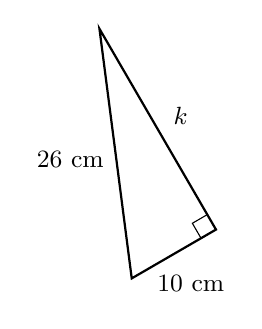
\begin{tikzpicture}[thick]
\draw (1.48,0.62)--(0,3.17)--(0.41,0)--cycle;
\draw[thin] (1.37,0.81)--(1.18,0.7)--(1.29,0.51);
\node at (1.03,2.06) {\small $k$};
\node at (1.16,-0.06) {\small 10 cm};
\node at (-0.37,1.51) {\small 26 cm};
\end{tikzpicture}}}\hfill\parbox[t]{11.6cm}{\textbf{029}\quad Berechne die fehlende Seite.\\[2pt]{\color{gray}\footnotesize rechnen · tripel, lage-gedreht, gesucht-kathete, andere-buchstaben · kern\\Ergebnis: $k = 24$ cm}}
\end{minipage}\par\medskip\hrule\medskip
\begin{minipage}[t]{\linewidth}
\parbox[t]{5.8cm}{\adjustbox{max width=5.5cm,max height=4.2cm,valign=t}{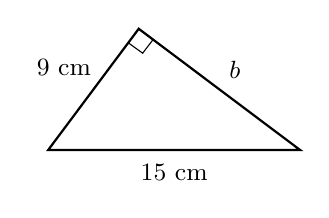
\begin{tikzpicture}[thick]
\draw (1.15,1.54)--(0,0)--(3.2,0)--cycle;
\draw[thin] (1.02,1.36)--(1.2,1.23)--(1.33,1.4);
\node at (0.2,1.05) {\small 9 cm};
\node at (2.37,1.02) {\small $b$};
\node at (1.6,-0.28) {\small 15 cm};
\end{tikzpicture}}}\hfill\parbox[t]{11.6cm}{\textbf{030}\quad Berechne die fehlende Seite.\\{\color{gray}\footnotesize a) grau: $b^2 = 15^2 - 9^2$ \quad $b^2 = 144 \quad | \sqrt{\ }$ \quad $b = 12$ cm}\\[2pt]{\color{gray}\footnotesize rechnen · tripel, hyp-waagerecht, gesucht-kathete, abc · kern\\Ergebnis: $b = 12$ cm}}
\end{minipage}\par\medskip\hrule\medskip
\begin{minipage}[t]{\linewidth}
\parbox[t]{5.8cm}{\adjustbox{max width=5.5cm,max height=4.2cm,valign=t}{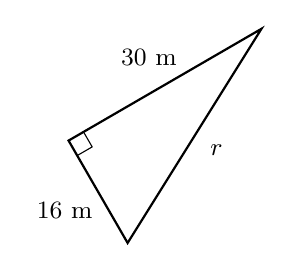
\begin{tikzpicture}[thick]
\draw (0,1.3)--(0.75,0)--(2.45,2.72)--cycle;
\draw[thin] (0.11,1.11)--(0.3,1.22)--(0.19,1.41);
\node at (-0.05,0.41) {\small 16 m};
\node at (1.02,2.36) {\small 30 m};
\node at (1.88,1.18) {\small $r$};
\end{tikzpicture}}}\hfill\parbox[t]{11.6cm}{\textbf{031}\quad Berechne die fehlende Seite.\\[2pt]{\color{gray}\footnotesize rechnen · tripel, lage-gedreht, gesucht-hyp, andere-buchstaben · kern\\Ergebnis: $r = 34$ m}}
\end{minipage}\par\medskip\hrule\medskip
\begin{minipage}[t]{\linewidth}
\parbox[t]{5.8cm}{\adjustbox{max width=5.5cm,max height=4.2cm,valign=t}{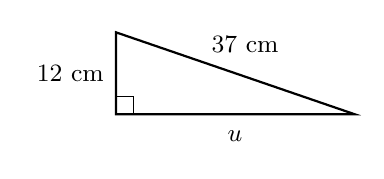
\begin{tikzpicture}[thick]
\draw (0,0)--(3.03,0)--(0,1.04)--cycle;
\draw[thin] (0.22,0)--(0.22,0.22)--(0,0.22);
\node at (1.51,-0.28) {\small $u$};
\node at (-0.58,0.52) {\small 12 cm};
\node at (1.64,0.88) {\small 37 cm};
\end{tikzpicture}}}\hfill\parbox[t]{11.6cm}{\textbf{032}\quad Berechne die fehlende Seite.\\[2pt]{\color{gray}\footnotesize rechnen · tripel, lage-standard, gesucht-kathete, andere-buchstaben · kern\\Ergebnis: $u = 35$ cm}}
\end{minipage}\par\medskip\hrule\medskip
\begin{minipage}[t]{\linewidth}
\parbox[t]{5.8cm}{\adjustbox{max width=5.5cm,max height=4.2cm,valign=t}{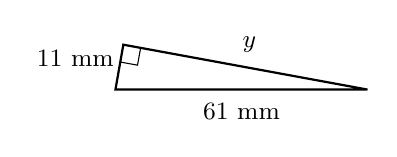
\begin{tikzpicture}[thick]
\draw (0.1,0.57)--(0,0)--(3.2,0)--cycle;
\draw[thin] (0.06,0.35)--(0.28,0.31)--(0.32,0.53);
\node at (-0.51,0.39) {\small 11 mm};
\node at (1.7,0.57) {\small $y$};
\node at (1.6,-0.28) {\small 61 mm};
\end{tikzpicture}}}\hfill\parbox[t]{11.6cm}{\textbf{033}\quad Berechne die fehlende Seite.\\[2pt]{\color{gray}\footnotesize rechnen · tripel, hyp-waagerecht, gesucht-kathete, andere-buchstaben · kern\\Ergebnis: $y = 60$ mm}}
\end{minipage}\par\medskip\hrule\medskip
\clearpage
\section*{Stufe 5 – Berechnen und runden}
\begin{minipage}[t]{\linewidth}
\parbox[t]{5.8cm}{\adjustbox{max width=5.5cm,max height=4.2cm,valign=t}{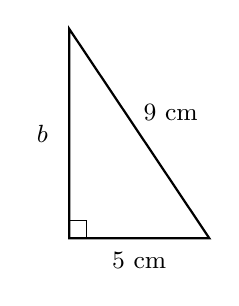
\begin{tikzpicture}[thick]
\draw (0,0)--(1.78,0)--(0,2.66)--cycle;
\draw[thin] (0.22,0)--(0.22,0.22)--(0,0.22);
\node at (0.89,-0.28) {\small 5 cm};
\node at (-0.34,1.33) {\small $b$};
\node at (1.29,1.6) {\small 9 cm};
\end{tikzpicture}}}\hfill\parbox[t]{11.6cm}{\textbf{034}\quad Berechne die fehlende Seite. Runde auf eine Stelle nach dem Komma.\\[2pt]{\color{gray}\footnotesize rechnen · krumm, lage-standard, gesucht-kathete, abc, einheit-gleich · kern\\Ergebnis: $b \approx 7{,}5$ cm}}
\end{minipage}\par\medskip\hrule\medskip
\begin{minipage}[t]{\linewidth}
\parbox[t]{5.8cm}{\adjustbox{max width=5.5cm,max height=4.2cm,valign=t}{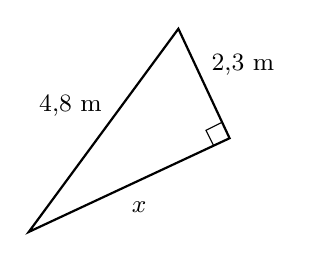
\begin{tikzpicture}[thick]
\draw (2.55,1.19)--(0,0)--(1.9,2.58)--cycle;
\draw[thin] (2.35,1.09)--(2.25,1.29)--(2.45,1.39);
\node at (1.4,0.32) {\small $x$};
\node at (2.72,2.12) {\small 2{,}3 m};
\node at (0.53,1.6) {\small 4{,}8 m};
\end{tikzpicture}}}\hfill\parbox[t]{11.6cm}{\textbf{035}\quad Berechne die fehlende Seite. Runde auf eine Stelle nach dem Komma.\\[2pt]{\color{gray}\footnotesize rechnen · dezimal, lage-gedreht, gesucht-kathete, andere-buchstaben, einheit-gleich · kern\\Ergebnis: $x \approx 4{,}2$ m}}
\end{minipage}\par\medskip\hrule\medskip
\begin{minipage}[t]{\linewidth}
\parbox[t]{5.8cm}{\adjustbox{max width=5.5cm,max height=4.2cm,valign=t}{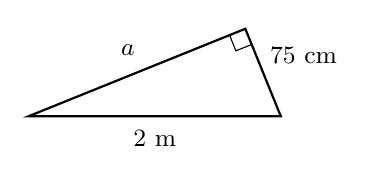
\begin{tikzpicture}[thick]
\draw (2.75,1.11)--(0,0)--(3.2,0)--cycle;
\draw[thin] (2.55,1.03)--(2.63,0.83)--(2.83,0.91);
\node at (1.26,0.84) {\small $a$};
\node at (3.49,0.77) {\small 75 cm};
\node at (1.6,-0.28) {\small 2 m};
\end{tikzpicture}}}\hfill\parbox[t]{11.6cm}{\textbf{036}\quad Berechne die fehlende Seite. Runde auf eine Stelle nach dem Komma.\\[2pt]{\color{gray}\footnotesize rechnen · einheit-gemischt, hyp-waagerecht, gesucht-kathete, abc · kern\\Ergebnis: $a \approx 185{,}4$ cm}}
\end{minipage}\par\medskip\hrule\medskip
\begin{minipage}[t]{\linewidth}
\parbox[t]{5.8cm}{\adjustbox{max width=5.5cm,max height=4.2cm,valign=t}{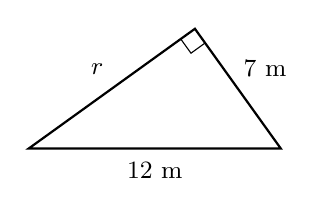
\begin{tikzpicture}[thick]
\draw (2.11,1.52)--(0,0)--(3.2,0)--cycle;
\draw[thin] (1.93,1.39)--(2.06,1.21)--(2.24,1.34);
\node at (0.87,1.01) {\small $r$};
\node at (3,1.01) {\small 7 m};
\node at (1.6,-0.28) {\small 12 m};
\end{tikzpicture}}}\hfill\parbox[t]{11.6cm}{\textbf{037}\quad Berechne die fehlende Seite. Runde auf eine Stelle nach dem Komma.\\[2pt]{\color{gray}\footnotesize rechnen · krumm, hyp-waagerecht, gesucht-kathete, andere-buchstaben, einheit-gleich · kern\\Ergebnis: $r \approx 9{,}7$ m}}
\end{minipage}\par\medskip\hrule\medskip
\begin{minipage}[t]{\linewidth}
\parbox[t]{5.8cm}{\adjustbox{max width=5.5cm,max height=4.2cm,valign=t}{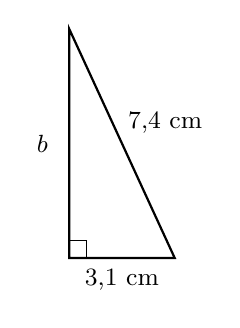
\begin{tikzpicture}[thick]
\draw (0,0)--(1.34,0)--(0,2.91)--cycle;
\draw[thin] (0.22,0)--(0.22,0.22)--(0,0.22);
\node at (0.67,-0.28) {\small 3{,}1 cm};
\node at (-0.34,1.45) {\small $b$};
\node at (1.22,1.71) {\small 7{,}4 cm};
\end{tikzpicture}}}\hfill\parbox[t]{11.6cm}{\textbf{038}\quad Berechne die fehlende Seite. Runde auf eine Stelle nach dem Komma.\\[2pt]{\color{gray}\footnotesize rechnen · dezimal, lage-standard, gesucht-kathete, abc, einheit-gleich · kern\\Ergebnis: $b \approx 6{,}7$ cm}}
\end{minipage}\par\medskip\hrule\medskip
\begin{minipage}[t]{\linewidth}
\parbox[t]{5.8cm}{\adjustbox{max width=5.5cm,max height=4.2cm,valign=t}{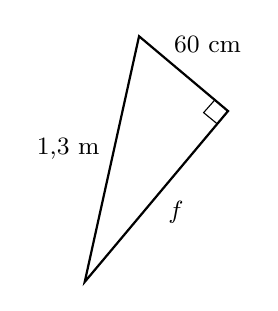
\begin{tikzpicture}[thick]
\draw (1.82,2.17)--(0.69,3.12)--(0,0)--cycle;
\draw[thin] (1.66,2.32)--(1.51,2.15)--(1.68,2.01);
\node at (1.56,3.01) {\small 60 cm};
\node at (1.16,0.88) {\small $f$};
\node at (-0.21,1.69) {\small 1{,}3 m};
\end{tikzpicture}}}\hfill\parbox[t]{11.6cm}{\textbf{039}\quad Berechne die fehlende Seite. Runde auf eine Stelle nach dem Komma.\\[2pt]{\color{gray}\footnotesize rechnen · einheit-gemischt, lage-gedreht, gesucht-kathete, andere-buchstaben · kern\\Ergebnis: $f \approx 115{,}3$ cm}}
\end{minipage}\par\medskip\hrule\medskip
\begin{minipage}[t]{\linewidth}
\parbox[t]{5.8cm}{\adjustbox{max width=5.5cm,max height=4.2cm,valign=t}{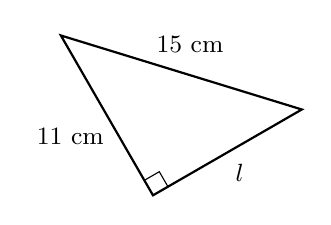
\begin{tikzpicture}[thick]
\draw (1.17,0)--(0,2.03)--(3.06,1.09)--cycle;
\draw[thin] (1.06,0.19)--(1.25,0.3)--(1.36,0.11);
\node at (0.12,0.75) {\small 11 cm};
\node at (2.27,0.28) {\small $l$};
\node at (1.64,1.91) {\small 15 cm};
\end{tikzpicture}}}\hfill\parbox[t]{11.6cm}{\textbf{040}\quad Berechne die fehlende Seite. Runde auf eine Stelle nach dem Komma.\\[2pt]{\color{gray}\footnotesize rechnen · krumm, lage-gedreht, gesucht-kathete, andere-buchstaben, einheit-gleich · kern\\Ergebnis: $l \approx 10{,}2$ cm}}
\end{minipage}\par\medskip\hrule\medskip
\begin{minipage}[t]{\linewidth}
\parbox[t]{5.8cm}{\adjustbox{max width=5.5cm,max height=4.2cm,valign=t}{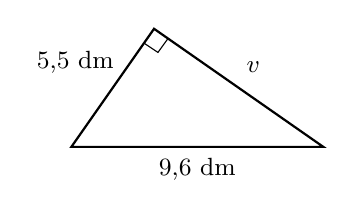
\begin{tikzpicture}[thick]
\draw (1.05,1.5)--(0,0)--(3.2,0)--cycle;
\draw[thin] (0.92,1.32)--(1.1,1.2)--(1.23,1.38);
\node at (0.05,1.08) {\small 5{,}5 dm};
\node at (2.31,1.01) {\small $v$};
\node at (1.6,-0.28) {\small 9{,}6 dm};
\end{tikzpicture}}}\hfill\parbox[t]{11.6cm}{\textbf{041}\quad Berechne die fehlende Seite. Runde auf eine Stelle nach dem Komma.\\[2pt]{\color{gray}\footnotesize rechnen · dezimal, hyp-waagerecht, gesucht-kathete, andere-buchstaben, einheit-gleich · kern\\Ergebnis: $v \approx 7{,}9$ dm}}
\end{minipage}\par\medskip\hrule\medskip
\begin{minipage}[t]{\linewidth}
\parbox[t]{5.8cm}{\adjustbox{max width=5.5cm,max height=4.2cm,valign=t}{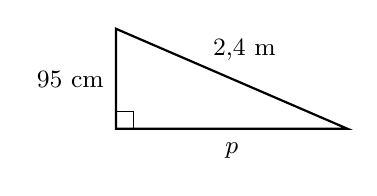
\begin{tikzpicture}[thick]
\draw (0,0)--(2.94,0)--(0,1.27)--cycle;
\draw[thin] (0.22,0)--(0.22,0.22)--(0,0.22);
\node at (1.47,-0.28) {\small $p$};
\node at (-0.58,0.63) {\small 95 cm};
\node at (1.63,1) {\small 2{,}4 m};
\end{tikzpicture}}}\hfill\parbox[t]{11.6cm}{\textbf{042}\quad Berechne die fehlende Seite. Runde auf eine Stelle nach dem Komma.\\[2pt]{\color{gray}\footnotesize rechnen · einheit-gemischt, lage-standard, gesucht-kathete, andere-buchstaben · kern\\Ergebnis: $p \approx 220{,}4$ cm}}
\end{minipage}\par\medskip\hrule\medskip
\clearpage
\section*{Stufe 6 – Sache, steigend}
\begin{minipage}[t]{\linewidth}
\parbox[t]{5.8cm}{\adjustbox{max width=5.5cm,max height=4.2cm,valign=t}{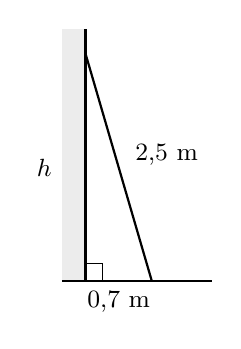
\begin{tikzpicture}[thick]
\fill[gray!15] (-0.3,0) rectangle (0,3.2); \draw (0,0)--(0,3.2);
\draw (-0.3,0)--(1.6,0);
\draw (0.84,0)--(0,2.88);
\draw[thin] (0,0.22)--(0.22,0.22)--(0.22,0);
\node[right] at (0.5,1.6) {\small 2,5 m};
\node[below] at (0.42,0) {\small 0,7 m};
\node[left] at (-0.3,1.44) {\small $h$};
\end{tikzpicture}}}\hfill\parbox[t]{11.6cm}{\textbf{043}\quad Eine 2,5 m lange Leiter lehnt an einer Wand. Ihr Fuß steht 0,7 m von der Wand weg. Berechne, wie hoch die Leiter reicht.\\[2pt]{\color{gray}\footnotesize sache · gesucht-kathete, einheit-gleich · kern\\Ergebnis: $h = 2{,}4$ m}}
\end{minipage}\par\medskip\hrule\medskip
\begin{minipage}[t]{\linewidth}
\parbox[t]{5.8cm}{\adjustbox{max width=5.5cm,max height=4.2cm,valign=t}{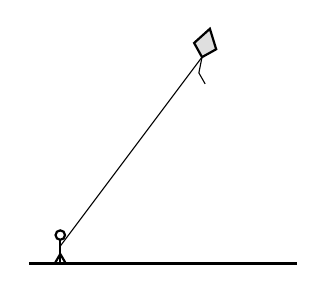
\begin{tikzpicture}[thick]
\draw (-0.4,0)--(3.0,0);
\draw (0,0)--(0,0.12); \draw (0,0.12)--(-0.07,0) (0,0.12)--(0.07,0);
\draw (0,0.12)--(0,0.3); \draw (0,0.36) circle (0.06);
\draw[thin] (0,0.22)--(1.8,2.62);
\draw[fill=gray!25] (1.8,2.62)--(1.98,2.72)--(1.9,2.98)--(1.7,2.8)--cycle;
\draw[thin] (1.8,2.62)--(1.76,2.42)--(1.84,2.28);
\end{tikzpicture}}}\hfill\parbox[t]{11.6cm}{\textbf{044}\quad Paul lässt einen Drachen steigen. Die Schnur ist 50 m lang und straff gespannt. Paul hält sie in 1,5 m Höhe. Der Punkt am Boden genau unter dem Drachen ist 30 m von Paul entfernt. Berechne, wie hoch der Drachen fliegt.\\[2pt]{\color{gray}\footnotesize sache · gesucht-kathete, falle-zusatzstrecke, einheit-gleich · kern\\Ergebnis: $41{,}5$ m}}
\end{minipage}\par\medskip\hrule\medskip
\begin{minipage}[t]{\linewidth}
\parbox[t]{5.8cm}{\parbox[t]{5.5cm}{\color{gray}\small (ohne Skizze)}}\hfill\parbox[t]{11.6cm}{\textbf{045}\quad Ein rechteckiger Spiegel hat eine Diagonale von 140 cm. Er ist 122 cm breit. Berechne, wie hoch er ist. Runde auf eine Stelle nach dem Komma.\\[2pt]{\color{gray}\footnotesize sache · gesucht-kathete, einheit-gleich · kern\\Ergebnis: $\approx 68{,}7$ cm}}
\end{minipage}\par\medskip\hrule\medskip
\begin{minipage}[t]{\linewidth}
\parbox[t]{5.8cm}{\adjustbox{max width=5.5cm,max height=4.2cm,valign=t}{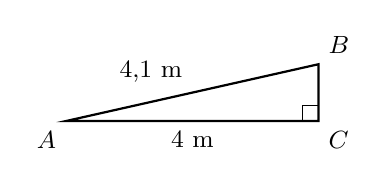
\begin{tikzpicture}[thick]
\draw (0,0)--(3.2,0)--(3.2,0.72)--cycle;
\draw[thin] (3.0,0)--(3.0,0.2)--(3.2,0.2);
\node[below left] at (0,0) {\small $A$};
\node[below right] at (3.2,0) {\small $C$};
\node[above right] at (3.2,0.72) {\small $B$};
\node[above left] at (1.6,0.36) {\small 4,1 m};
\node[below] at (1.6,0) {\small 4 m};
\end{tikzpicture}}}\hfill\parbox[t]{11.6cm}{\textbf{046}\quad Eine Rampe führt auf eine Bühne. Die Rampe $\overline{AB}$ ist 4,1 m lang, am Boden überbrückt sie $\overline{AC} = 4$ m. Berechne die Höhe $\overline{BC}$ der Bühne.\\[2pt]{\color{gray}\footnotesize sache · gesucht-kathete, streckennamen, einheit-gleich · kern\\Ergebnis: $\overline{BC} = 0{,}9$ m}}
\end{minipage}\par\medskip\hrule\medskip
\begin{minipage}[t]{\linewidth}
\parbox[t]{5.8cm}{\adjustbox{max width=5.5cm,max height=4.2cm,valign=t}{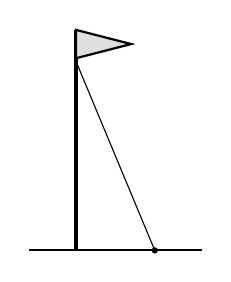
\begin{tikzpicture}[thick]
\draw (-0.6,0)--(1.6,0);
\draw[line width=1.6pt] (0,0)--(0,2.8);
\draw[fill=gray!25] (0,2.8)--(0.7,2.62)--(0,2.44)--cycle;
\draw[thin] (0,2.4)--(1.0,0);
\fill (1.0,0) circle (0.04);
\end{tikzpicture}}}\hfill\parbox[t]{11.6cm}{\textbf{047}\quad Ein Fahnenmast ist mit einem straffen Seil abgespannt. Das Seil ist 13 m lang und 500 cm vom Fuß des Mastes im Boden verankert. Berechne, in welcher Höhe das Seil am Mast befestigt ist.\\[2pt]{\color{gray}\footnotesize sache · gesucht-kathete, einheit-gemischt · kern\\Ergebnis: $12$ m}}
\end{minipage}\par\medskip\hrule\medskip
\begin{minipage}[t]{\linewidth}
\parbox[t]{5.8cm}{\parbox[t]{5.5cm}{\color{gray}\small (ohne Skizze)}}\hfill\parbox[t]{11.6cm}{\textbf{048}\quad Das Seil einer Seilbahn ist 1,3 km lang und gerade gespannt. Waagerecht überbrückt es 1,2 km. Die Talstation liegt auf 650 m Höhe. Berechne, auf welcher Höhe die Bergstation liegt.\\[2pt]{\color{gray}\footnotesize sache · gesucht-kathete, falle-zusatzstrecke, einheit-gemischt · kern\\Ergebnis: $1150$ m}}
\end{minipage}\par\medskip\hrule\medskip
\begin{minipage}[t]{\linewidth}
\parbox[t]{5.8cm}{\adjustbox{max width=5.5cm,max height=4.2cm,valign=t}{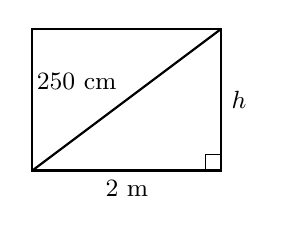
\begin{tikzpicture}[thick]
\draw (0,0) rectangle (2.4,1.8);
\draw (0,0)--(2.4,1.8);
\draw[thin] (2.2,0)--(2.2,0.2)--(2.4,0.2);
\node[below] at (1.2,0) {\small 2 m};
\node[above left] at (1.2,0.9) {\small 250 cm};
\node[right] at (2.4,0.9) {\small $h$};
\end{tikzpicture}}}\hfill\parbox[t]{11.6cm}{\textbf{049}\quad Ein rechteckiges Gartentor ist 2 m breit. Die schräge Strebe von Ecke zu Ecke ist 250 cm lang. Berechne die Höhe $h$ des Tores.\\[2pt]{\color{gray}\footnotesize sache · gesucht-kathete, rechteck-diagonale, einheit-gemischt · kern\\Ergebnis: $h = 150$ cm}}
\end{minipage}\par\medskip\hrule\medskip
\begin{minipage}[t]{\linewidth}
\parbox[t]{5.8cm}{\adjustbox{max width=5.5cm,max height=4.2cm,valign=t}{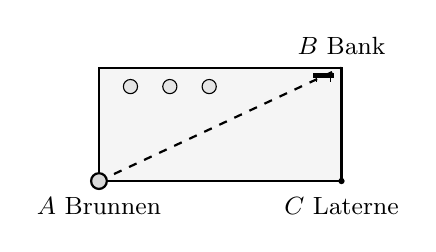
\begin{tikzpicture}[thick]
\draw[fill=gray!8] (0,0) rectangle (3.08,1.44);
\draw[dashed] (0,0)--(3.08,1.44);
\draw[fill=gray!30] (0,0) circle (0.1);
\draw[line width=1.5pt] (2.72,1.34)--(2.98,1.34);
\draw[thin] (2.76,1.34)--(2.76,1.26) (2.94,1.34)--(2.94,1.26);
\fill (3.08,0) circle (0.04); \draw (3.08,0)--(3.08,0.22);
\foreach \x in {0.4,0.9,1.4} \draw[thin,fill=gray!20] (\x,1.2) circle (0.09);
\node[below] at (0,-0.08) {\small $A$ Brunnen};
\node[below] at (3.08,-0.08) {\small $C$ Laterne};
\node[above] at (3.08,1.48) {\small $B$ Bank};
\end{tikzpicture}}}\hfill\parbox[t]{11.6cm}{\textbf{050}\quad Ein Platz ist rechteckig. Vom Brunnen $A$ führt ein gerader Weg quer über den Platz zur Bank $B$; er ist 85 m lang. Am Rand entlang sind es von $A$ bis zur Laterne $C$ 77 m. Berechne die Länge $\overline{BC}$.\\[2pt]{\color{gray}\footnotesize sache · gesucht-kathete, streckennamen, einheit-gleich · kern\\Ergebnis: $\overline{BC} = 36$ m}}
\end{minipage}\par\medskip\hrule\medskip
\begin{minipage}[t]{\linewidth}
\parbox[t]{5.8cm}{\parbox[t]{5.5cm}{\color{gray}\small (ohne Skizze)}}\hfill\parbox[t]{11.6cm}{\textbf{051}\quad Ein 3,4 m langes Brett lehnt an einer Mauer. Unten steht es 1,8 m von der Mauer weg, oben ragt es 40 cm über die Mauerkante hinaus. Berechne, wie hoch die Mauer ist.\\[2pt]{\color{gray}\footnotesize sache · gesucht-kathete, falle-zusatzstrecke, einheit-gemischt · kern\\Ergebnis: $2{,}4$ m}}
\end{minipage}\par\medskip\hrule\medskip
\clearpage
\section*{Stufe 7 – Ziel (P10)}
\begin{minipage}[t]{\linewidth}
\parbox[t]{5.8cm}{\parbox[t]{5.5cm}{\color{gray}\small (ohne Skizze)}}\hfill\parbox[t]{11.6cm}{\textbf{052}\quad Ein gerades Förderband soll Pakete auf eine Rampe in 315 cm Höhe bringen. Sein unteres Ende liegt 134 cm über dem Boden. Das Band ist 625 cm lang, waagerecht überbrückt es 600 cm. Entscheide mit einer Rechnung, ob das obere Ende die Rampe erreicht.\\[2pt]{\color{gray}\footnotesize sache · dreistellig, gesucht-kathete, falle-hyp-addiert, falle-zusatzstrecke, einheit-gleich · ziel\\Ergebnis: Nein, oberes Ende auf $309$ cm}}
\end{minipage}\par\medskip\hrule\medskip
\begin{minipage}[t]{\linewidth}
\parbox[t]{5.8cm}{\adjustbox{max width=5.5cm,max height=4.2cm,valign=t}{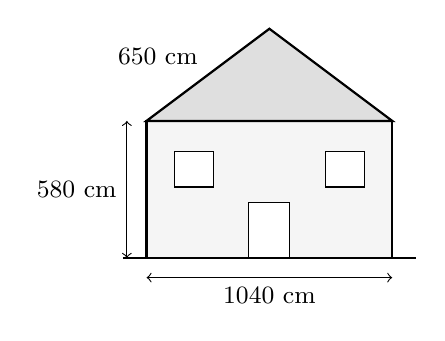
\begin{tikzpicture}[thick]
\draw (-0.3,0)--(3.42,0);
\draw[fill=gray!8] (0,0) rectangle (3.12,1.74);
\draw[fill=gray!25] (0,1.74)--(1.56,2.91)--(3.12,1.74)--cycle;
\draw[thin,fill=white] (1.3,0) rectangle (1.82,0.7);
\draw[thin,fill=white] (0.35,0.9) rectangle (0.85,1.35);
\draw[thin,fill=white] (2.27,0.9) rectangle (2.77,1.35);
\draw[thin,<->] (0,-0.25)--(3.12,-0.25); \node[below] at (1.56,-0.25) {\small 1040 cm};
\draw[thin,<->] (-0.25,0)--(-0.25,1.74); \node[left] at (-0.25,0.87) {\small 580 cm};
\node[above left] at (0.78,2.33) {\small 650 cm};
\end{tikzpicture}}}\hfill\parbox[t]{11.6cm}{\textbf{053}\quad Ein Haus ist 1040 cm breit, seine Wände sind 580 cm hoch. Die Dachsparren sind 650 cm lang und treffen sich in der Mitte am First. Der Bebauungsplan erlaubt höchstens 10 m bis zum First. Entscheide mit einer Rechnung, ob das Haus so gebaut werden darf.\\[2pt]{\color{gray}\footnotesize sache · dreistellig, gesucht-kathete, falle-hyp-addiert, falle-zusatzstrecke, einheit-gleich · ziel\\Ergebnis: Ja, First bei $970$ cm}}
\end{minipage}\par\medskip\hrule\medskip
\begin{minipage}[t]{\linewidth}
\parbox[t]{5.8cm}{\parbox[t]{5.5cm}{\color{gray}\small (ohne Skizze)}}\hfill\parbox[t]{11.6cm}{\textbf{054}\quad Ein Fernseher hat eine Bildschirmdiagonale von 165 cm, der Bildschirm ist 85 cm hoch. Das Fach im Regal ist 145 cm breit und 90 cm hoch. Entscheide mit einer Rechnung, ob der Bildschirm in das Fach passt (der Rand des Geräts zählt nicht).\\[2pt]{\color{gray}\footnotesize sache · dreistellig, gesucht-kathete, falle-hyp-addiert, einheit-gleich · ziel\\Ergebnis: Ja, Breite $\approx 141{,}4$ cm}}
\end{minipage}\par\medskip\hrule\medskip
\begin{minipage}[t]{\linewidth}
\parbox[t]{5.8cm}{\adjustbox{max width=5.5cm,max height=4.2cm,valign=t}{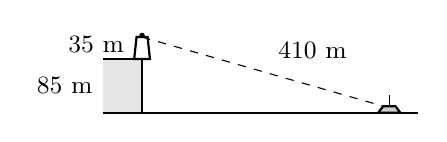
\begin{tikzpicture}[thick]
\draw[fill=gray!20] (-0.5,0)--(0,0)--(0,0.68)--(-0.5,0.68);
\draw (-0.5,0)--(3.5,0);
\draw[fill=white] (-0.1,0.68)--(-0.07,0.96)--(0.07,0.96)--(0.1,0.68)--cycle;
\fill (0,0.98) circle (0.035);
\draw[dashed,thin] (0,0.96)--(3.14,0.06);
\draw[fill=gray!40] (3.0,0)--(3.28,0)--(3.22,0.08)--(3.06,0.08)--cycle;
\draw[thin] (3.14,0.08)--(3.14,0.22);
\node[left] at (-0.5,0.34) {\small 85 m};
\node[left] at (-0.1,0.86) {\small 35 m};
\node[above right] at (1.6,0.55) {\small 410 m};
\end{tikzpicture}}}\hfill\parbox[t]{11.6cm}{\textbf{055}\quad Ein Leuchtturm ist 35 m hoch und steht auf einer 85 m hohen Klippe. Vom Licht oben bis zu einem Boot sind es in gerader Linie 410 m. Boote müssen mindestens 400 m Abstand vom Fuß der Klippe halten. Entscheide mit einer Rechnung, ob das Boot genug Abstand hat.\\[2pt]{\color{gray}\footnotesize sache · dreistellig, gesucht-kathete, falle-hyp-addiert, falle-zusatzstrecke, einheit-gleich · ziel\\Ergebnis: Nein, Abstand $\approx 392{,}1$ m}}
\end{minipage}\par\medskip\hrule\medskip
\end{document}
